\section{2. Предел числовой последовательности: единственность, ограниченность. Переход к пределу в неравенствах. Теорема о зажатой последовательности. Арифметические операции с пределами. Бесконечные пределы. Теорема о пределе монотонной последовательности. Теорема Кантора о вложенных отрезках. Теорема Больцано--Вейерштрасса. Частичные пределы, теорема о верхнем и нижнем пределах. Фундаментальные последовательности и критерий Коши.}

    \begin{definition}
        Число $a$ называется пределом последовательности $\{a_{n}\}$, если
        \[\forall \epsilon > 0 \ \exists N \in \N \ \forall n \in \N \ (n \geq N \Rightarrow |a_{n}-a| < \epsilon)\]
        Пишут $\lim_{n \to \infty} a_{n} = a$, или $a_{n} \to a$ при $n \to \infty$, или $a_{n} \to a$.
    \end{definition}
    
    \begin{theorem}{Теорема о единственности.}
        \\
        Если $\lim_{n \to \infty} a_{n} = a$ и $\lim_{n \to \infty} a_{n} = b$, то $a = b$.
    \end{theorem}
    
    \begin{proof}
        Пусть $a \neq b$, тогда $|a-b| > 0$. Положим, $\epsilon = \frac{|a-b|}{2}$, тогда:\\
        $\exists N_1 \ \forall n \geq N_{1} (|a_{n} - a| < \epsilon)$\\
        $\exists N_2 \ \forall n \geq N_{2} (|a_{n} - b| < \epsilon)$\\
        Положим $N = max\{N_{1}, N_{2}\}$, тогда:
        \[|a-b| = |a-a_{N}+a_{N}-b| \leq |a_{N}-a| + |a_{N}-b| < \epsilon + \epsilon = |a-b|\]
        Противоречие.
    \end{proof}

    \begin{theorem}{Теорема об ограниченности.}
        \\
        Если последовательность $\{a_{n}\}$ сходится, то она ограничена.
    \end{theorem}

    \begin{proof}
        Пусть $a_{n} \rightarrow a \in \R$.\\
        По определению предела $(\epsilon = 1)$:
        \[\exists N \in \N \ \forall n \geq N(a-1 < a_{n} < a+1)\]
        Положим, $m = min\{a-1, a_{1}, ..., a_{N-1}\}$, $M = max\{a+1, a_{1}, ..., a_{N-1}\}$.\\
        Тогда $\forall n \in \N \ (m \leq a_{n} \leq M)$.
    \end{proof}

    \begin{theorem}{О пределе в неравенствах.}
        \\
        Пусть $\lim_{n \to \infty} a_{n} = a$, $\lim_{n \to \infty} b_{n} = b$. Тогда:\\
        1) $a < b \Rightarrow \exists N \in \N \ \forall n > N \ (a_{n} < b_{n})$\\
        2) $\exists n_0 \in \N \ \forall n \geq n_0 \ (a_{n} \leq b_{n}) \Rightarrow a \leq b$
    \end{theorem}

    \begin{proof} \ \\
        1) Положим $\epsilon = \frac{b-a}{2}$.\\
        Тогда $\epsilon > 0$ и по определению предела:\\
        $\exists N_1 \in \N : \forall n \geq N (a_{n} < a+\epsilon)$\\
        $\exists N_2 \in \N : \forall n \geq N (b_{n} > b-\epsilon)$\\
        Положим $N = max\{N_1, N_2\}$.\\
        Тогда при $n \geq N$ имеем $a_{n} < a+\epsilon = \frac{a+b}{2} = b-\epsilon  < b_{n}$.\\
        2) Второе утверждение вытекает из первого по правилу контрапозиции.
    \end{proof}
    
    \begin{note}
        Предельный переход не обязан сохранять строгие неравенства:\\
        Пример: $a_{n} = 0, b_{n} = \frac{1}{n} \Rightarrow \forall n \in \N \ (0 < \frac{1}{n})$, но $\lim_{n \to \infty} a_{n} = \lim_{n \to \infty} b_{n} = 0$.
    \end{note}

    \begin{theorem}{О зажатой последовательности.}
        \\
        Пусть $a_{n} \leq c_{n} \leq b_{n}$ для всех $n \geq n_0$, и $\lim_{n \to \infty} a_{n} = a$, $\lim_{n \to \infty} b_{n} = a$, тогда существует $\lim_{n \to \infty} c_{n} = a$.
    \end{theorem}

    \begin{proof}
        Зафиксируем $\epsilon > 0$. По определению предела:\\
        $\exists N_1 \in \N \ \forall n \geq N_1 \ (a-\epsilon < a_{n})$\\
        $\exists N_2 \in \N \ \forall n \geq N_2 \ (b_{n} < a+\epsilon)$.\\
        Положим $N = max\{N_1, N_2, n_{0}\}$, тогда при $n \geq N$ имеем:
        \[a-\epsilon < a_{n} \leq c_{n} \leq b_{n} < a+\epsilon \Rightarrow |c_{n} - a| < \epsilon \Rightarrow \lim_{n \to \infty} c_{n} = a\]
    \end{proof}

    \begin{theorem}{Об арифметических операциях с пределами.}
        \\
        Пусть $\lim_{n \to \infty} a_{n} = a$, $\lim_{n \to \infty} b_{n} = b$, тогда:
        \begin{enumerate}
            \item $\lim_{n \to \infty}(a_{n} + b_{n}) = a+b$
            \item $\lim_{n \to \infty}(a_{n} \cdot b_{n}) = a \cdot b$
            \item $b \neq 0, \forall n \in \N \ (b_{n} \neq 0) \Rightarrow \lim_{n \to \infty}(\frac{a_{n}}{b_{n}}) = \frac{a}{b}$
        \end{enumerate}
    \end{theorem}

    \begin{proof} \
        \begin{enumerate}
        \item Зафиксируем $\epsilon > 0$. По определению предела:\\
            $\exists N_1 \in \N \ n \geq N_1 \ (|a_{n}-a| < \frac{\epsilon}{2})$\\
            $\exists N_2 \in \N \ n \geq N_2 \ (|b_{n}-b| < \frac{\epsilon}{2})$\\
            Положим $N = max\{N_1, N_2\}$, тогда\\
            $\forall n \geq N$ $|(a_{n} + b_{n}) - (a + b)| \leq |a_{n} - a| + |b_{n} - b| < \frac{\epsilon}{2} + \frac{\epsilon}{2} = \epsilon$
        
        \item Так как $\{a_{n}\}$ -- сходящаяся, то $\{a_{n}\}$ -- ограниченная, то есть $\exists C > 0$, что $\forall n \in \N \ (|a_{n}| \leq C)$. Увеличивая $C$, если необходимо, можно считать, что $|b| \leq C$.\\
            Зафиксируем $\epsilon > 0$. По определению предела\\
            $\exists N_1 \ \forall n \geq N_1 \ (|a_{n} - a| < \frac{\epsilon}{2C})$\\
            $\exists N_2 \ \forall n \geq N_2 \ (|b_{n} - b| < \frac{\epsilon}{2C})$\\
            Положим $N = max\{N_1, N_2\}$, тогда при $n \geq N$ имеем:\\
            $|a_{n}b_{n} - ab| = |a_{n}b_{n} - a_{n}b + a_{n}b - ab| \leq |a_{n}||b_{n} - b| + |b||a_{n} - a| < C\frac{\epsilon}{2C} + C\frac{\epsilon}{2C} = \epsilon$
   
        \item Так как $\frac{a_{n}}{b_{n}} = a_{n} \cdot \frac{1}{b_{n}}$, тогда по пункту 2 достаточно показать, что $\lim_{n \to \infty} \frac{1}{b_{n}} = \frac{1}{b}$.\\
            Поскольку $|b| \neq 0$, то по определению предела:\\
            $\exists N_1 \in \N \ \forall n \geq N_1 \ (|b_{n} - b| < \frac{|b|}{2})$. При этом $|b| = |b - b_{n} + b_{n}| \leq |b_{n} - b| + |b_{n}| < \frac{|b|}{2} + |b_{n}|$,\\
            откуда $|b_{n}| > \frac{|b|}{2}$.\\
            Зафиксируем $\epsilon > 0$. По определению предела:\\
            $\exists N_2 \in \N \ \forall n \geq N_2 \ (|b_{n} - b| < \frac{\epsilon|b|^2}{2})$\\
            Положим $N = max\{N_1, N_2\}$. Тогда при $n \geq N$ имеем $|\frac{1}{b_{n}} - \frac{1}{b}| = \frac{|b_{n} - b|}{|b||b_{n}|} < \frac{2}{|b|^2} \cdot \epsilon \cdot \frac{|b|^2}{2} = \epsilon$
        \end{enumerate}
    \end{proof}

    \begin{definition}
        1) Говорят, что $\{a_{n}\}$ \textit{стремится} к $+ \infty$, если 
        \[\forall \epsilon > 0 \  \exists n_{0} \in \N \ \forall n \in \N \ (n \geq n_{0} \Rightarrow a_{n} > \frac{1}{\epsilon})\]
        Пишут $\lim_{n \to \infty} a_{n} = + \infty$ или $ a_{n} \rightarrow + \infty$.
        \\
        2) Говорят, что $\{a_{n}\}$ \textit{стремится} к $- \infty$, если 
        \[\forall \epsilon > 0 \  \exists n_{0} \in \N \ \forall n \in \N \ (n \geq n_{0} \Rightarrow a_{n} < \frac{-1}{\epsilon})\]
        Пишут $\lim_{n \to \infty} a_{n} = - \infty$ или $ a_{n} \rightarrow - \infty$.
        \\
        3) Последовательность $a_{n}$ называется бесконечно большой (б.б.), если $\lim_{n \to \infty} a_{n} = \infty$
    \end{definition}
    
    \textbf{Замечание.} Если последовательность имеет предел в $\overline{\R}$, то он единственный.

    \begin{theorem}{О пределе монотонной последовательности}
        \\
        1) Если последовательность $\{a_{n}\}$ нестрого возрастает, то существует $\lim_{n \to \infty} a_{n} = sup\{a_{n}\}$. Если к тому же $\{a_{n}\}$ ограничена сверху, то $\{a_{n}\}$ -- сходящаяся.
        \\
        2) Если последовательность $\{a_{n}\}$ нестрого убывает, то существует $\lim_{n \to \infty} a_{n} = inf\{a_{n}\}$. Если к тому же $\{a_{n}\}$ ограничена снизу, то $\{a_{n}\}$ -- сходящаяся.
    \end{theorem}
    
    \begin{proof}
        1) Пусть $\{a_{n}\}$ ограничена сверху. Тогда $c = sup\{a_{n}\} \in \R$. Зафиксируем $\epsilon > 0$. По определению супремума выполнено:
        $\begin{cases}
            \forall n \in \N (a_{n} \leq c)
            \\
            \exists N \in \N (a_{N} > c - \epsilon)
        \end{cases}$
        \\
        В силу возрастания при $n \geq N$:
        \[c - \epsilon < a_{N} \leq a_{n} \leq c < c + \epsilon\]
        Значит, $|a_{n} - c| < \epsilon$. Т.к. $\epsilon > 0$ -- любое, то $c = \lim_{n \to \infty} a_{n}$.
        \\
        Пусть $\{a_{n}\}$ неограничена сверху, $sup\{a_{n}\} = + \infty$. Зафиксируем $\epsilon > 0$. Тогда $\exists N \in \N (a_{N} > \frac{1}{\epsilon})$ и в силу возрастания $a_{n} \geq a_{N} > \frac{1}{\epsilon} \ \forall n \geq N \Rightarrow \lim_{n \to \infty} a_{n} = + \infty$.
        \\
        2) Аналогично пункту 1.
    \end{proof}

    \begin{definition}
        Последовательность отрезков $\{[a_{n}, b_{n}]\}$ называется \textit{вложенной}, если $[a_{n}, b_{n}] \supset [a_{n+1}, b_{n+1}] \ \forall n \in \N$.
        Если к тому же $\{b_{n}-a_{n}\} \to 0$, то $\{[a_{n}, b_{n}]\}$ называется \textit{стягивающейся}.
    \end{definition}

    \begin{theorem}{Теорема Кантора}\\
        Всякая последовательность вложенных отрезков имеет общую точку. Если последовательность стягивающейся, то такая точка единственная.
    \end{theorem}
    
    \begin{center}
        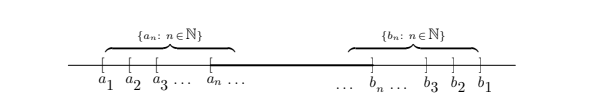
\includegraphics[width=0.7\textwidth]{colloq2.png}
    \end{center}

    \begin{proof}
        Пусть $\{[a_{n}, b_{n}]\}$ -- последовательность вложенных отрезков.\\
        Поскольку $a_1 \leq a_{n} \leq a_{n+1} \leq b_{n+1} \leq b_{n} \leq b_1 \ \forall n$, то \\
        $\{a_{n}\}$ -- нестрого возрастает и ограничена сверху числом $b_1$,\\
        $\{b_{n}\}$ -- нестрого убывает и ограничена снизу числом $a_1$.\\
        По теореме о пределе монотонной последовательности обе последовательности сходятся $a_{n} \to \alpha$ и $b_{n} \to \beta$.
        
        Переходя в неравенстве $a_{n} \leq b_{n} \ \forall n$ к пределу при $n \to \infty$, получим $\alpha \leq \beta$. Ввиду монотонности $a_{n} \leq \alpha \leq \beta \leq b_{n} \ \forall n$, следовательно $\cap_{n = 1}^{\infty}[a_{n}, b_{n}] \supset [\alpha, \beta]$, значит $\cap_{n = 1}^{\infty}[a_{n}, b_{n}] \neq \emptyset$.
        
        Пусть $\{[a_{n}, b_{n}]\}$ -- стягивающаяся, и $x, y \in \cap_{n = 1}^{\infty} [a_{n}, b_{n}]$. Так как $x, y \in [a_{n}, b_{n}] \ \forall n \Rightarrow |x-y| \leq b_{n} - a_{n} \ \forall n$. Переходя к пределу при $n \rightarrow \infty$, получим $x = y$, то есть $\cap_{n = 1}^{\infty}[a_{n}, b_{n}] = \{x\}$, где $x = \alpha = \beta$.
    \end{proof}

    \begin{definition}
        Пусть $\{a_{n}\}$ -- последовательность, $\{n_{k}\}$ -- строго возрастающая последовательность натуральных чисел. Последовательность $\{b_{k}\}$, где $b_{k} = a_{n_{k}} \ \forall k$, называется \textit{подпоследовательностью} $\{a_{n}\}$ и обозначается $\{a_{n_{k}}\}$.
    \end{definition}
    
    \begin{theorem}{Больцано -- Вейерштрасса}\\
        Всякая ограниченная последовательность имеет сходящуюся подпоследовательность.
    \end{theorem}

    \begin{proof}
        Пусть $\{a_{n}\}$ -- ограничена, тогда $a_{n} \in [c, d] \ \forall n$.\\
        Положим $[c_1, d_1] = [c, d]$.\\
        Положим $y = \frac{c_{1}+d_{1}}{2}$, тогда:\\
        $[c_{k+1}, d_{k+1}] = \begin{cases}
            [c_{k}, y]$, если $\{m: a_{m} \in [c_{k}, y]\}$ -- бесконечно$\\
            [y, d_{k}]$ - иначе$
        \end{cases}$

        По индукции будет построена последовательность вложенных отрезков $[c_{k}, d_{k}]$, каждый из которых содержит значения бесконечного множества членов $a_{n}$.\\
        По теореме Кантора (о вложенных отрезках) существует общая точка $a = \lim_{k \to \infty} c_{k} = \lim_{k \to \infty} d_{k}$.\\
        Построим строго возрастающую последовательность номеров $\{n_{k}\}$.\\
        Положим $n_1 = 1$, если номер $n_{k}$ найден, то выберем номер $n_{k+1} > n_{k}$ так, что $a_{n_{k+1}} \in [c_{k+1}, d_{k+1}]$.
        Т.к. по построению $c_{k} \leq a_{n_{k}} \leq d_{k} \ \forall k$, то по теореме о зажатой последовательности $\{a_{n_{k}}\} \rightarrow a$.
    \end{proof}

    \begin{definition}
        Точка $a \in \overline{\R}$ называется \textit{частичным пределом} последовательности $\{a_{n}\}$, если \ \ \ \ $a$ -- предел некоторой подпоследовательности $\{a_{n_{k}}\}$.
    \end{definition}

    Для последовательности $\{a_{n}\}$ определим $M_{k} = \sup_{n \geq k}\{a_{n}\}$, $m_{k} = inf_{n \geq k}\{a_{n}\}$. Так как при переходе к подмножеству, $\sup$ не увеличивается, а $\inf$ не уменьшается, то имеем следующую цепочку неравенств:
    \[m_{k} \leq m_{k+1} \leq M_{k+1} \leq M_{k} \  \forall k\]
    Cледовательно, $\{m_{k}\}$ нестрого возрастает, а $\{M_{k}\}$ нестрого убывает, и значит, эти последовательности имеют предел в $\overline{\R}$.
    
    \begin{note}
        Если $\{a_{n}\}$ не ограничена сверху (снизу), то $M_{k} = +\infty \ (m_{k} = -\infty) \ \forall k$. Будем считать, что $\lim_{k \to \infty} M_{k} = +\infty \ (\lim_{k \to \infty} m_{k} = -\infty)$.
    \end{note}

    \begin{definition} \ \\
        $\overline{\lim_{n \to \infty}} a_{n} = \lim_{k \to \infty} \sup_{n \geq k}\{a_{n}\}$ называется \textit{верхним пределом} $\{a_{n}\}$\\
        $\underline{\lim_{n \to \infty}} a_{n} = \lim_{k \to \infty} \inf_{n \geq k}\{a_{n}\}$ называется \textit{нижним пределом} $\{a_{n}\}$\\
    \end{definition}

    \begin{theorem}
        Верхний (нижний) предел -- это наибольший (наименьший) из частичных пределов последовательности в $\overline{\R}$.
    \end{theorem}

    \begin{proof}
        $M = \overline{\lim_{n \to \infty}} a_{n}$, $m = \underline{\lim_{n \to \infty}} a_{n}$\\
        Нужно показать, что $m, M$ -- частичные пределы и все частичные пределы лежат между $[m, M]$.\\
        Докажем, что $M$ -- это частичный предел $\{a_{n}\}$:
        \begin{enumerate}
            \item 
            Пусть $M \in \R$. Так как $M-1 < M_1 = \sup\{a_{n}\}_{n = 1}^{+\infty}$, то существует $n_1$ такой, что $M-1 < a_{n_1} \leq M_{n_{1}}$. Так как $M - \frac{1}{2} < M_{n_1 + 1} = \sup_{n \geq n_1+1}\{a_{n}\}$, то существует номер $n_2 > n_1$ такой, что $M - \frac{1}{2} < a_{n_2} \leq M_{n_2}$ и т.д.\\
            По индукции будет построена подпоследовательность $\{a_{n_{k}}\}$, такая что\\
            $M-\frac{1}{k} < a_{n_{k}} \leq M_{n_{k}} \ \forall k$.\\
            Поскольку $\lim_{k \to \infty} (M - \frac{1}{k}) = \lim_{k \to \infty} (M_{n_{k}}) = M$, то по теореме о зажатой последовательности $\{a_{n_{k}}\} \to M$.
            \item 
            Пусть $M = +\infty \Rightarrow M_{k} = +\infty \ \forall k$.\\
            Так как $\{a_{n}\}$ не ограничена сверху, то существует номер $n_1$, такой что $1 < a_{n_1}$.\\
            Так как $\{a_{n}\}$ не ограничена сверху, то существует $n_2$, такой что $2 < a_{n_2}$.\\
            По индукции будет построена $\{a_{n}\}$, такая что $k < a_{n_{k}}$. Так как последовательность $\{k\}_{k = 1}^{\infty} \to +\infty$, то $a_{n_{k}} \to +\infty$.
            \item 
            Пусть $M = -\infty$. Так как $a_{k} \leq M_{k} \ \forall k$\\
            $M_{k} \to -\infty$, то $a_{k} \to -\infty$.
        \end{enumerate}
        В любом из случаев $M$ -- частичный предел $\{a_{n}\}$.\\
        Доказательство для $m$ аналогично.\\
        Пусть $a$ -- частичный предел $\{a_{n}\}$, $a_{n_{k}} \rightarrow a$. Т.к. $n_{k} \geq k$, то 
            \[m_{k} \leq a_{n_{k}} \leq M_{k} \  \forall k\]
            Перейдем к пределу при $k \rightarrow \infty$. Получим $m \leq a \leq M$.
    \end{proof}

    \begin{definition}
        Последовательность $a_{n}$ называется \textit{фундаментальной}, если
        \[\forall \epsilon > 0 \ \exists N \in \N \ \forall n, m \in \N (n \geq N, m \geq N \Rightarrow |a_{n} - a_{m}| < \epsilon)\]
    \end{definition}
    
    \begin{lemma}
        Всякая фундаментальная последовательность ограничена.
    \end{lemma}
    
    \begin{proof}
        Пусть $\{a_{n}\}$ фундаментальна. Тогда
        \[\exists N \ \forall n, m \geq N (|a_{n} - a_{m}| < 1)\]
        В частности, $\forall n \geq N \ (a_{N} - 1 < a_{n} < a_{N} + 1)$.
        Положим $\alpha = min\{a_{1}, ..., a_{N-1}, a_{N} - 1\}, \beta = max\{a_{1}, ..., a_{N-1}, a_{N} + 1\}$, тогда $\alpha \leq a_n \leq \beta \ \forall n \in \N$.
    \end{proof}
    
    \begin{theorem}{Критерий Коши.}\\
     Последовательность $\{a_{n}\}$ сходится тогда и только тогда, когда она фундаментальна.
    \end{theorem}
    
    \begin{proof}
        1) Пусть $a_{n} \rightarrow a \in \R$. Зафиксируем $\epsilon > 0$. По определению предела $\exists N \\ \forall n \geq N \ (|a_{n} - a| < \frac{\epsilon}{2})$. Тогда при $n, m \geq N$
        \[|a_{n} - a_{m}| = |(a_{n} - a) + (a - a_{m})| \leq |a_{n} - a| + |a_{m} - a| < \frac{\epsilon}{2} + \frac{\epsilon}{2} = \epsilon.\]
        Значит, последовательность $\{a_{n}\}$ -- фундаментальна.
        \\
        2) Пусть $\{a_{n}\}$ фундаментальна. По лемме \{$a_{n}\}$ ограничена. Тогда по теореме Больцано-Вейерштрасса:
        \[\exists \{a_{n_{k}}\}, a_{n_{k}} \rightarrow a\]
        Покажем, что $a = \lim_{n \to \infty} a_{n}$. Зафиксируем $\epsilon > 0$. По определению фундаментальной последовательности $\exists N \ \forall n,m \geq N (|a_{n} - a_{m}| < \frac{\epsilon}{2})$. Покажем, что $N$ -- подходящий номер в определении предела $\{a_{n}\}$ для $\epsilon$. В силу сходимости $\{a_{n_{k}}\}$ $\exists K \ \forall k \geq K \ (|a_{n_{k}} - a| < \frac{\epsilon}{2})$. Положим $M = max\{N, K\}$. Тогда $n_{M} \geq M \geq N, n_{M} \geq M \geq K$ и, значит, при $n \geq N$:
        \[|a_{n} - a| \leq |a_{n} - a_{n_{M}}| + |a_{n_{M}} - a| < \frac{\epsilon}{2} + \frac{\epsilon}{2} = \epsilon.\]
        Так как $\epsilon > 0$, то $a = \lim_{n \to \infty} a_{n}$.
    \end{proof}